%%%%%%%%%%%%%%%%%%%%%%%%%%%%%%%%%%%%%%%%%%%%%%
%                                            %
%    Dyussenov Nuraly BSc Thesis Work        %
%                                            %
%%%%%%%%%%%%%%%%%%%%%%%%%%%%%%%%%%%%%%%%%%%%%%

\documentclass[12pt,a4paper,oneside]{book} % twoside,openany

% Packages
\usepackage[T1]{fontenc}
\usepackage[utf8]{inputenc}

\usepackage{amsmath,amssymb,amsthm}
\usepackage{cancel}
\usepackage{enumerate}
\usepackage{graphicx}
\usepackage{caption,subcaption}
\graphicspath{{./figures/}}

\usepackage{array}
\newcolumntype{L}[1]{>{\raggedright\let\newline\\\arraybackslash\hspace{0pt}}m{#1}}
\newcolumntype{C}[1]{>{\centering\let\newline\\\arraybackslash\hspace{0pt}}m{#1}}
\newcolumntype{R}[1]{>{\raggedleft\let\newline\\\arraybackslash\hspace{0pt}}m{#1}}

\usepackage{url  }
\usepackage{hyperref}
\usepackage{tikz}
\usetikzlibrary{decorations.pathreplacing}

\setlength {\marginparwidth }{2cm}

\usepackage{todonotes}

\usepackage{setspace}

% Theoremlike environment
\newtheorem{theorem}{Theorem}[section]
\newtheorem{proposition}[theorem]{Proposition}
\newtheorem{lemma}[theorem]{Lemma}
\newtheorem{corollary}[theorem]{Corollary}
\newtheorem{remark}[theorem]{Remark}
\newtheorem{definition}[theorem]{Definition}
\newtheorem{example}[theorem]{Example}
\newtheorem{assumption}[theorem]{Assumption}

% Ususal abbreviations
\newcommand{\N}{\mathbb{N}}
\newcommand{\Z}{\mathbb{Z}}
\newcommand{\Q}{\mathbb{Q}}
\newcommand{\R}{\mathbb{R}}

% Probability theory
\newcommand{\A}{\mathcal{A}}
\newcommand{\B}{\mathcal{B}}
\newcommand{\C}{\mathcal{C}}
\newcommand{\F}{\mathcal{F}}
\newcommand{\G}{\mathcal{G}}
\newcommand{\X}{\mathcal{X}}
\newcommand{\Y}{\mathcal{Y}}
\newcommand{\M}{\mathcal{M}}
\renewcommand{\P}{\mathbb{P}}
\newcommand{\E}{\mathbb{E}}
\newcommand{\D}{\mathbb{D}}
\newcommand{\law}[1]{\text{Law}(#1)}

\newcommand{\Var}{\mathrm{Var}}

\newcommand{\Cov}{\mathrm{Cov}}

\newcommand{\Pas}{\text{a.s.}}
\newcommand{\ind}{\mathds{1}}

% Analysis
\newcommand{\eps}{\varepsilon}
\newcommand{\la}{\lambda}
\newcommand{\ga}{\gamma}
\newcommand{\ka}{\kappa}
\newcommand{\dtv}{d_{\text{TV}}}

% Integration
\newcommand{\dint}{\mathrm{d}} 

\newcommand{\lfrf}[1]{\lfloor #1\rfloor}


%%%%%%%%%%%%%%%%%%%%%%%%%%%%%%%%%%%%55% Page layout
\usepackage{indentfirst}
%\usepackage{fullpage}
\usepackage[a4paper]{geometry}
% \geometry{tmargin=3cm,lmargin=3.5cm,rmargin=2cm}
% manual page formatting
%\setlength{\headsep}{25pt}
\hyphenation{}

% headers and footers
\usepackage{fancyhdr}
\usepackage{mathptmx}

\newcommand\HRule{\rule{\textwidth}{1pt}}

\usepackage{varwidth}

%\usepackage{booktabs}
\usepackage{multirow,array}
\usepackage{siunitx}

% Quotations
\usepackage{csquotes}

\makeatletter
\renewcommand{\@chapapp}{}% Not necessary...
\newenvironment{chapquote}[2][2em]
{\setlength{\@tempdima}{#1}%
	\def\chapquote@author{#2}%
	\parshape 1 \@tempdima \dimexpr\textwidth-2\@tempdima\relax%
	\itshape}
{\par\normalfont\hfill--\ \chapquote@author\hspace*{\@tempdima}\par\bigskip}
\makeatother



\newcommand{\code}[1]{\texttt{#1}}


\usepackage{titlesec, blindtext, color}
\definecolor{gray75}{gray}{0.75}
\newcommand{\hsp}{\hspace{20pt}}


\newcommand{\stdwidth}{0.61\linewidth}

% Space above chapter titles
\usepackage{titlesec}

\renewcommand{\baselinestretch}{1.5}



\begin{document}
\onehalfspacing

\begin{titlepage}
	
	%\newcommand{\HRule}{\rule{\linewidth}{0.5mm}} % Defines a new command for the horizontal lines, change thickness here
	
	\center % Center everything on the page
	
	%----------------------------------------------------------------------------------------
	%	HEADING SECTIONS
	%----------------------------------------------------------------------------------------
	
	\textsc{\LARGE Budapesti University of Technology and Economics}\\[1.5cm] % Name of your university/college
	\textsc{\Large Institute of Mathematics}\\[0.5cm] % Major heading such as course name
	\textsc{\large Bachelor Thesis}\\[0.5cm] % Minor heading such as course title
	
	%----------------------------------------------------------------------------------------
	%	TITLE SECTION
	%----------------------------------------------------------------------------------------
	
	\HRule \\[0.4cm]
	{ \Large \bfseries Linear Regression through Origin
		 }\\[0.4cm]
	\HRule \\[1.5cm]
	
	%----------------------------------------------------------------------------------------
	%	AUTHOR SECTION
	%----------------------------------------------------------------------------------------
	
	\begin{tabular}{L{6cm} R{8cm}}
	\emph{Author:}   & \emph{Supervisor:} \\
	Dyussenov Nuraly & Dr. Jozsef Mala   \\
	                 & Associate Professor, BME Fac. of Nat. Sci. 
	\end{tabular}\\[1.3cm]

	
	\vfill
	{\Large Budapest, \today}\\[1.2cm] % Date, change the \today to a set date if you want to be precise
		
	
\includegraphics[trim={0cm 0cm 0cm 0cm},clip,width=0.5\linewidth]{bme_logo_nagy.eps}
	 % Include a department/university logo - this will require the graphicx package
	
	%\vfill % Fill the rest of the page with whitespace
	
\end{titlepage}

	%\newpage\null\thispagestyle{empty}\newpage

	\frontmatter
	%\chapter*{\centering Kivonat}
	
	\tableofcontents
	%\listoftables
	%\listoffigures
		
	\mainmatter
	
	\fancypagestyle{plain}{%

		\fancyhf{}
		\fancyhead[L]{\rule[-2ex]{0pt}{2ex}\small \leftmark} 
		\fancyhead[R]{} 
		\fancyfoot[L]{}
		\fancyfoot[C]{-- \thepage\ --}
		\fancyfoot[R]{} 
		\renewcommand{\headrulewidth}{1.5pt}
		\renewcommand{\footrulewidth}{1pt}}
	\pagestyle{plain}
	
	\titleformat{\chapter}[display]{\normalfont\huge\bfseries}{\chaptertitlename\ \thechapter}{20pt}{\Huge}
	\titlespacing*{\chapter}{10pt}{20pt}{40pt}
	 
	\titleformat{\chapter}[hang]{\Huge\bfseries}{\thechapter.\hsp}{0pt}{\Huge\bfseries} 
	  
	\chapter{Preliminaries} 
	
	\begin{chapquote}{Name of the author} % Quotation (optional)
	''A place for future inspirational quote.''
	\end{chapquote}


	\section{Introduction}

% Start your introduction with a general statement about linear regression through the origin

In the world of regression analysis, choosing the right model is a constant challenge, balancing simplicity and accuracy. This thesis focuses on a specific aspect—linear regression through the origin (RTO) —examining its statistical properties when dealing with just one explanatory variable. Our goal is to identify situations where this approach might be more suitable than the commonly used simple linear regression. Through this study, we aim to shed light on the conditions that make regression through the origin a preferable choice, offering insights that bridge mathematical rigor with real-world applicability. Join us on this journey as we navigate the complexities of statistical modeling, striving to understand when and why regression through the origin might outperform its more conventional counterpart.

	\subsection*{Simple Linear Regression}

Before we start delving into RTO, it's best to get familiar with a more general case - Simple Linear Regression.

In Simple Linear Regression, we are given a random sample of data points $(x_1,y_1),...,(x_n,y_n)$ from a population, and our goal is to find a linear function


\begin{equation}\label{eq:lin}
	y = \beta_1 x + \beta_o
\end{equation}

That describes the relationship between two variables $x$ and $y$ as good as possible. Since, sample is random, the equation \eqref{eq:lin} is not true in general, so we take into account the error term $\epsilon$:

\begin{equation}\label{eq:lin2}
	y = \beta_1 x + \beta_o + \epsilon
\end{equation}


The objective of simple linear regression is, under some \todo{List out the conditions} conditions*, to estimate the parameters $\beta_0$ and $\beta_1$, so that they will provide best fit. 


Likelihood function
\[
L(y_1, \ldots, y_n | \beta_0, \beta_1, \sigma) = \left( \frac{1}{2\pi\sigma^2} \right)^{n/2} \exp\left( -\frac{1}{2\sigma^2} \sum_{i=1}^{n} (y_i - (\beta_0 + \beta_1 x_i))^2 \right)
\]

Log-likelihood function
\[
l(y_1, \ldots, y_n | \beta_0, \beta_1, \sigma) = c - n \log \sigma - \frac{1}{2\sigma^2} \sum_{i=1}^{n} (y_i - (\beta_0 + \beta_1 x_i))^2
\]


% Equations
\begin{align}
	\frac{\partial l}{\partial \beta_0} &= \sum_{i=1}^{n} (y_i - (\beta_0 + \beta_1 x_i)) = 0 \label{eq:est_beta_0} \\
	\frac{\partial l}{\partial \beta_1} &= \sum_{i=1}^{n} (y_i - (\beta_0 + \beta_1 x_i))x_i = 0 \label{eq:est_beta_1} \\
	\frac{\partial l}{\partial \sigma} &= \frac{n}{\sigma} - \frac{1}{\sigma^3} \sum_{i=1}^{n} (y_i - (\beta_0 + \beta_1 x_i))^2 = 0 
\end{align}
	

% Text
Let the solutions of the above equations be denoted as $\hat{\beta}_0$, $\hat{\beta}_1$, $\hat{\sigma}^2$ for $\beta_0$, $\beta_1$, $\sigma^2$. If $\hat{y}_i = \hat{\beta}_0 + \hat{\beta}_1 x_i$, then...

% Equations
\begin{align*}
\hat{\beta}_0  &= \bar{y} - \hat{\beta}_1 \bar{x}; \\
\hat{\beta}_1 &= \frac{S_{xy}}{S_{xx}}; \\
\hat{\sigma}^2 &= \frac{1}{n} \sum_{i=1}^{n} (y_i - \hat{y}_i)^2 = \frac{1}{n} SSE.
\end{align*}

So $\hat{\beta}_0, \hat{\beta}_1$ are Maximum Likelikelihood Estimators of the model.

\begin{proposition}
	Finding values of $\beta_0, \beta_1 $ that minimize MSE is same as finding MLE of $\beta_0 ,\beta_1 $
\end{proposition}


\begin{proof}
	\todo{todo}
\end{proof}



% Proposition and Proof
\textbf{Proposition}
\[
\sum_{i=1}^{n} (y_i - \bar{y})^2 = \sum_{i=1}^{n} (\hat{y}_i - \bar{y})^2 + \sum_{i=1}^{n} (y_i - \hat{y}_i)^2
\]

% Proof (continued)
\begin{proof}The vector $\textbf{y} - \textbf{$\hat{y}$}$ is perpendicular to $\textbf{$\hat{y}$} - \textbf{1 $\bar{y}$}$, thus the proposition is true by the Pythagorean theorem.

Alternatively, it is enough to show that

\[
	\sum (\hat{y}_i-\bar{y})(y_i-\hat{y}_i) = 0	
\],

since then:

\begin{align*}
	\sum_{i=1}^{n} (y_i - \bar{y})^2 &= (\sum_{i=1}^{n} (\hat{y}_i - \bar{y}) + \sum_{i=1}^{n} (y_i - \hat{y}_i))^2 = \\
	&= \sum_{i=1}^{n} (\hat{y}_i - \bar{y})^2 + 2\sum (\hat{y}_i-\bar{y})(y_i-\hat{y}_i)+ \sum_{i=1}^{n} (y_i - \hat{y}_i)^2 = \\
	&= \sum_{i=1}^{n} (\hat{y}_i - \bar{y})^2 + \sum_{i=1}^{n} (y_i - \hat{y}_i)^2 \\
\end{align*}

From \ref{eq:est_beta_0} we know that $\sum (y_i=\bar{y}_i)=0$.
From \ref{eq:est_beta_1} we know that $\sum (y_i-\hat{y}_i)x_i=0$,
$\hat{y}_i = \beta_0 + \beta_1 x_i \Rightarrow x_i = \frac{1}{\beta_1}(\hat{y}_i-\beta_0) \Rightarrow \sum \hat{y}_i (y_i-\hat{y}_i)=0$

Finally, 

\[
	\sum (\hat{y}_i-\bar{y})(y_i-\hat{y}_i) = \sum \hat{y}_i(y_i-\hat{y}_i)-\bar{y}\sum (y_i-\hat{y}_i)=0	
\]


\end{proof}


% Proposition
\textbf{Proposition 1.4.} The estimators $\hat{\beta}_0$, $\hat{\beta}_1$, $\frac{SSE}{n-2}$ are unbiased estimators of $\beta_0$, $\beta_1$, $\sigma^2$ respectively.



% Proof that the estimators are unbiased
\textbf{Proof:}

1. \textbf{Unbiasedness of $\hat{\beta}_1$:}
\[
\mathbb{E} [ \hat{\beta _1} ] = \mathbb{E} [\frac{S_{xy}}{S_{xx}}] = \mathbb{E} [\frac{\Sigma (x_i - \bar{x})(y_i-\bar{y})}{\Sigma (x_i-\bar{x})^2}]=
\]

\[
	= \mathbb{E} [\frac{\Sigma (x_i - \bar{x})y_i}{\Sigma (x_i-\bar{x})^2}]=
	\frac{\Sigma (x_i - \bar{x})\mathbb{E} [y_i]}{\Sigma (x_i-\bar{x})^2}=
\]

\[
	= \frac{\Sigma (x_i - \bar{x})(\beta_0+\beta_1x_i)}{\Sigma (x_i-\bar{x})^2}=	
	\frac{\Sigma (x_i \beta_0 - \bar{x}\beta_0+\beta_1x_i^2-\beta_1x_i\bar{x})}{\Sigma x_i^2-n\bar{x}^2}=
\]

\[
	= \frac{\cancel{n\bar{x}\beta_0}-\cancel{n\bar{x}\beta_0}+\Sigma\beta_1x_i^2-n\beta_1\bar{x}^2}{\Sigma x_i^2-n\bar{x}^2}= \frac{(\Sigma x_i^2-n\bar{x}^2)\beta_1}{\Sigma x_i^2-n\bar{x}^2} = \beta_1
\]


2. \textbf{Unbiasedness of $\hat{\beta}_0$:}
\[
\mathbb{E}(\hat{\beta}_0) = \mathbb{E}(\bar{y} - \hat{\beta}_1 \bar{x}) = \bar{y} - \bar{x} \mathbb{E}(\hat{\beta}_1) = \frac{1}{n}\mathbb{E}[\Sigma y_i]-\beta_1 \bar{x} =
\] 

\[
	= \frac{1}{n}\mathbb{E}[\Sigma (\beta_0+\beta_1x_i)]-\beta_1 \bar{x} 
	= \frac{1}{n}n\beta_0+\frac{1}{n}n\beta_1\bar{x}-\bar{x}\beta_1=\beta_0	
\]


3. \textbf{Unbiasedness of $\frac{SSE}{n-2}$ as an estimator of $\sigma^2$:}
\[
\mathbb{E}\left(\frac{SSE}{n-2}\right) = \frac{1}{n-2} (n - 2) \sigma^2 = \sigma^2
\]


\begin{proposition}
	$\mathbb{V}ar[\hat{\beta}_1] = \frac{\sigma^2}{S_{xx}}$
\end{proposition}

\begin{proof}
	Assume, $Y_i \sim N(0, \sigma^2) $
	\[
		\mathbb{V}ar[\hat{\beta}_1] = \mathbb{V}ar (\frac{1}{S_{xx}}\sum (x_i-\bar{x})Y_i) = \frac{1}{S_{xx}^2}\sum \mathbb{V}ar Y_i = \frac{\sigma}{S_{xx}^2}
	\]
\end{proof}

	\clearpage





\chapter{Linear Regression Regression with no intercept term}

	\section{Simple Linear Regression with no intercept term}

	In certain statistical applications, the conventional assumption of a non-zero intercept term ($\beta_0$) in a simple linear regression model may not align with the nature of the data. For example, in economics the cost of production be assumed to be zero, when there is no production, or in physics, when we are describing the relationship between force and the displacement, forced is assumede to be zero, when there is no displacement.
	
	
	Likelihood function $L$ is:
	\begin{align*}
		L(y_1,...,y_n | \beta, \sigma) &= \prod \frac{1}{\sqrt{2 \pi \sigma^2}} \exp(-\frac{1}{2\sigma^2 (y_i-\beta x_i)^2}) \\
		&= \frac{1}{(2\pi \sigma^2)^{n/2}}\exp(-\frac{1}{2\sigma^2} \sum (y_i-\beta x_i)^2)
	\end{align*}

	Log-likelihood $l$ is:

\[
	l(y_1,...,y_n | \beta, \sigma)=-\frac{n}{2}\log(2\pi \sigma^2)-\frac{1}{2 \sigma^2} \sum (y_i - \beta x_i)^2
\]


\begin{align*}
	\frac{\partial l}{\partial \beta} = - \frac{1}{2 \sigma^2} & \sum 2(y_i-\beta x_i)(-x_i)=0 \\
	\frac{1}{\sigma^2}& \sum (y_i x_i - \beta x_i ^2) = 0 \\
	& \sum x_i y_i =  \sum  x_i^2 \beta \\
	& \hat{\beta} = \frac{\sum x_i y_i}{\sum x_i^2}
\end{align*}


	\begin{proposition}
		$\hat{\beta}$ is unbiased
	\end{proposition}

	\begin{proof}
		\begin{align*}
			\mathbb{E} [\hat{\beta}] &= \mathbb{E} [\frac{\sum x_i y_i}{\sum x_i^2}] = \sum \frac{1}{x_i^2} \mathbb{E}[\sum x_i y_i] = \\
			&= \frac{\sum x_i\mathbb{E}[y_i]}{\sum x_i^2} = \frac{\sum x_i^2 \beta}{\sum x_i^2} = \beta 
		\end{align*}
	\end{proof}


	\begin{proposition}
		$\mathbb{V}ar[\hat{\beta}_1^0] = \frac{\sigma^2}{\sum x_i^2}$
	\end{proposition}


	\begin{proof}
		\[
		\mathbb{V}ar[\hat{\beta}_1^0] =  \mathbb{V}ar[\frac{\sum x_i y_i}{\sum x_i^2}] = \frac{1}{(\sum x_i^2)^2} \sum x_i^2 \mathbb{V}ar[Y_i] = \frac{\sigma^2}{\sum x_i^2}
		\]
	\end{proof}


	\begin{proposition}
		\[
			\mathbb{V}ar[\hat{\beta}_1^0] < \mathbb{V}ar[\hat{\beta}_1]
		\]
	\end{proposition}

	\begin{proof}
		\begin{align*}
			\sum x_i^2 &> \sum (x_i - \bar{x})^2  \\
			\frac{1}{\sum x_i^2}  &< \frac{1}{\sum (x_i - \bar{x})^2}  \\
			\frac{\sigma^2}{\sum x_i^2}  &< \frac{\sigma^2}{\sum (x_i - \bar{x})^2}  \\
			\mathbb{V}ar[\hat{\beta}_1^0] &< \mathbb{V}ar[\hat{\beta}_1] 
		\end{align*}
	\end{proof}


This might suggest that $\hat{\beta}_1^0$ might be more accurate estimator than $\hat{\beta}_1$ for the slope term. This gives us some motivation to compare the two estimators more closely.

It would be convenient for us to find confidence interval for $\beta_1^0 - \beta_1$, since if 0 lies in the CI, then we can statistically infer that two estimators are very close.

\begin{proposition} \label{prop:normally}
	The difference of the two estimators is normally distributed as follows:
	\[
		\hat{\beta_1^0}-\hat{\beta_1} \sim N(\beta_1^0-\beta_1, \sigma^2(\frac{1}{S_{xx}}-\frac{1}{S_{xx}^0}))
	\]
\end{proposition}

	Before proving proposition \ref{prop:normally}, let's first understand some properties of $\hat{\beta_1^0}-\hat{\beta_1}$:

\begin{proposition}
	$\Cov (\hat{\beta_1^0},\hat{\beta_1^0}-\hat{\beta_1})=0$
\end{proposition}

\begin{proof}
	\begin{align*}
		\Cov (\hat{\beta_1^0},\hat{\beta_1^0}-\hat{\beta_1}) &=
		\Cov (\frac{\sum xy}{\sum x^2},\frac{\sum xy}{\sum x^2}-\frac{\sum (x-\bar{x})y}{\sum (x-\bar{x})^2})  \\
		&= \frac{\sum x^2}{(\sum x^2)^2} \Var\  y - \frac{\sum x(x-\bar{x})}{\sum x^2 \sum (x-\bar{x})^2} \Var \ y \\
		&=\sigma^2(\frac{1}{\sum x^2} - \frac{\sum x^2 - \bar{x}\sum x}{\sum x^2 \sum(x^2-2x\bar{x}+\bar{x}^2)}) \\
		&= \sigma^2 (\frac{1}{\sum x^2}-\frac{\sum x^2 - n \bar{x}^2}{\sum x^2(\sum x^2 - 2n\bar{x}^2+n\bar{x}^2)}) \\
		&=\sigma^2 (\frac{1}{\sum x^2}-\frac{\sum x^2 - n \bar{x}^2}{\sum x^2(\sum x^2 -n\bar{x}^2)}) \\
		&= \sigma^2(\frac{1}{\sum x^2}-\frac{1}{\sum x^2})=0
	\end{align*}
\end{proof}

\begin{proposition}
	$\E [\hat{\beta_1^0}-\hat{\beta_1}]=\beta_1^0-\beta_1$
\end{proposition}

\begin{proof}
	By linearity of expected value, $\E [\hat{\beta_1^0}-\hat{\beta_1}]= \E[\hat{\beta_1^0}] - \E[\hat{\beta_1}]= \beta_1^0-\beta_1 $
\end{proof}
	
	Now we are ready to prove proposition \ref{prop:normally}
\begin{proof}[Proof of prop. \ref{prop:normally}]
	$\hat{\beta_1^0}-\hat{\beta_1}$ is a linear combination of mutually independent normally distributed r.v.-s $\Rightarrow$ it is normally distributed.
	\todo{you can show that}
	
	\begin{align*}
		\Var (\hat{\beta_1^0}-\hat{\beta_1})&=\Var(\hat{\beta_1^0}) + \Var(\hat{\beta_1}) - 2 \Cov (\hat{\beta_1^0},\hat{\beta_1}) =\frac{\sigma^2}{S_{xx}^0}+\frac{\sigma^2}{S_{xx}}-2 \Cov (\hat{\beta_1^0},\hat{\beta_1^0}-\hat{\beta_1})-2 \Cov (\hat{\beta_1^0},\hat{\beta_1^0}) \\
		&= \frac{\sigma^2}{S_{xx}^0}+\frac{\sigma^2}{S_{xx}} - 0 -2 \Var \ \hat{\beta_1^0}=\frac{\sigma^2}{S_{xx}}-\frac{\sigma^2}{S_{xx}^0}
	\end{align*}
\end{proof}
	
Using proposition \ref{prop:normally}, we can now construct confidence interval for $\beta_1^0-\beta_1$:

\[
			\hat{\beta_1^0}-\hat{\beta_1} \sim N(\beta_1^0-\beta_1, \sigma^2(\frac{1}{S_{xx}}-\frac{1}{S_{xx}^0}))
\]

\[
	Z := \frac{\hat{\beta_1^0}-\hat{\beta_1}-\E [\hat{\beta_1^0}-\hat{\beta_1}]}{\Var (\hat{\beta_1^0}-\hat{\beta_1})}= \frac{\hat{\beta_1^0}-\hat{\beta_1}-(\beta_1^0-\beta_1)}{\sigma^2(\frac{1}{S_{xx}}-\frac{1}{S_{xx}^0})})
\]

\[
	\beta_1^0-\beta_1= \hat{\beta_1^0}-\hat{\beta_1} - \sigma^2 Z(\frac{1}{S_{xx}}-\frac{1}{S_{xx}^0})
\]

CI is:

\begin{equation}
\hat{\beta_1^0}-\hat{\beta_1} - \sigma^2 Z_{\alpha}(\frac{1}{S_{xx}}-\frac{1}{S_{xx}^0}) \leq \beta_1^0-\beta_1 \leq \hat{\beta_1^0}-\hat{\beta_1} + \sigma^2 Z_{\alpha}(\frac{1}{S_{xx}}-\frac{1}{S_{xx}^0})
\end{equation}






	\subsection{Motivational example}

Even though RTO might be worse than performing full linear regression model in terms of SSE (since full model always gives unbiased estimators, they are also MLE estimators, so SSE is minimized), there are other statistical parameters that are better in RTO when intercept term is small enough.

Given that the true model is known, $\dot{y_i} = \beta_1 x_i + \alpha$, one might simulate the data points by adding normally-distributed error terms:

\[
	y_i =  \beta_1 x_i + \alpha + \epsilon_i
\]

One might be interested now in comparing sum of squared deviations (SSD) of fitted points $\sum (\dot{y_i}-\hat{y_i})^2 $.

Let's start by generating a sample of 100 points, and assume that parameters are known as $\beta = 1, \alpha = 0.05$ (see fig. \ref{fig:simulation}):



\begin{figure}
	\begin{subfigure}{0.5\textwidth}
		\centering
		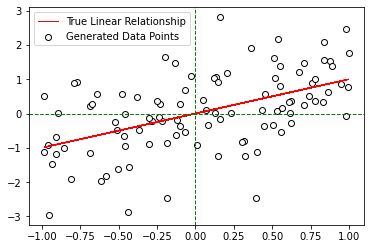
\includegraphics[width=\linewidth]{simulation.png}
		\caption{Plot of simulated points}
		\label{fig:simulation}
	\end{subfigure}%
	\begin{subfigure}{0.5\textwidth}
		\centering
		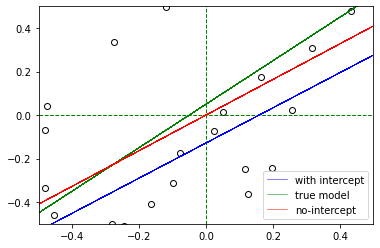
\includegraphics[width=\linewidth]{threemodels.png}
		\caption{Plot of three models}
		\label{fig:threemodels}
	\end{subfigure}
	\caption{Overall caption for the figure}
\end{figure}


Now, let's fit two models: no-intercept model, and full model. For that purposes we will use LinearRegression function from \code{sklearn.linear\_model} package. On fig. \ref{fig:threemodels} you can see the two models as well as the true model plotted up close.

Now let's compare two statistics for these two models: BIC (Bayesian Information Criterion) and SSD.

The results are as follows:

\begin{align*}
	BIC_{no} &= 386.1685814527955 \\
	BIC &= 391.09782858386046 \\
	SSD_{no} &= 1.2267420929010404 \\
	SSD &= 4.150248687009578	
\end{align*}


It is clearly seen that no-intercept model provides better fit in terms of these parameters.







	

\clearpage

	\subsection{Relevant Literature}
	Refer to seminal works and research studies that have explored or utilized the simple linear regression model without an intercept term. A brief review of the literature provides additional context and allows for a synthesis of existing knowledge in this specialized domain.



	\section{Comparative Analysis}	
	


	
	\clearpage

	
	\chapter{Applications to Linear Regression through Origin}


	\clearpage

	\section{Something to add 1} 

	
	\section{Something to add 1} 


	\chapter{Theoretical results} 
	
	\section{A theoretical resilt}
	
	\section{Towards some advanced topic}


	\chapter{Programming simulations} %


		
	\chapter{Summary and closing words}
	% 1 page
	



	% All in all 26-30 pages
	

	\bibliography{nuraly}
	\bibliographystyle{plain}
	
	\appendix
	
	\chapter{Program Codes}
	
\end{document}
